\chapter{Implementation}
The developped algorithm is written in Python coding language.\\
It was deemed appropriate to subdivide the whole script in five main modules in order to have a clean and modular package. This also allows for saving files with intermediate results to save computational power since some processes are very demanding.\\
Enumerating the modules :
\begin{itemize}
    \item \textbf{dataset split} into training and test set;
    \item \textbf{calculus} of the Line Spread Profile matrix \textbf{$Q_i$} for every image;
    \item \textbf{building} of the over-complete \textbf{dictionaries} $D_{SC}$ and $D_{RC}$;
    \item SVM \textbf{training}
    \item address the performane of the \textbf{SVC testing} it on the test set.
\end{itemize}
\paragraph{How to use} Sequence of action in order to make this code work:
\begin{enumerate}
    \item run 'phase1$\_$QiCalculusdataset.py' (no need to do that because they are already computed in the given complete$\_$dataset folder) : compute all the matrices for each camera and type of image;
    \item run 'dataset$\_$acquisition$\_$txt.py' : perform the training and test sets formation;
    \item run 'make$\_$dictionary$\_$from$\_$txt.py' or 'make$\_$dictionary$\_$from$\_$txt$\_$.py' : the only difference here is that in the first module the building process start with complitely empty dictionaries; instead in the second one, dictionaries are initialized;
    \item run 'SVM$\_$training.py' : compute and save the hyperplane equation which better  separates the plane linearly;
    \item run 'SVM$\_$classifier.py' : saves significant statistics about achieved performances ;
\end{enumerate}
\section{Dataset formation}
This module automatically splits the whole dataset into training and test set as explained in the \textit{Section VI-A} of the reference paper \cite{paper}.\\
As specified in the latter :
\begin{itemize}
    \item for single captured images, $15$ randomly chosen images are selected for training purposes;
    \item concerning recaptured images, for every pair of cameras involved, where the first one is the device used to capture the original image and the second one the system used to recapture it, we randomly select $3$ pictures for training purposes.
\end{itemize}
The remaining ones, both for recaptured and single captured images, are kept for performance testing.\\
For each camera, both in single captured and recaptured images, the outputs are two .txt files containing the paths of the Line Spread Profile matrices for training and test images respectively.
\section{$Q_i$ Calculus}
    In this section we implement the method described in the paper \cite{paper} for the calculus of the matrix $Q$.\\
    The proposed process determines, for any given single or recaptured image, a LSP matrix $Q_i$. 
    Since this part is very computationally demanding, we stored the resulting matrices in the corresponding directory of each camera model to used them later on in the next steps.\\

    The feature matrix extracted for each dataset's image contains the LSP of any columns presents in the selected blocks. We achieved these blocks by applying the following criterion, explained in details in the paper :
    \begin{itemize}
        \item firstly, the query image is converted to greyscale and all edges contained in the image are detected using a Canny Edge Detector (Canny Filter);
        \item the query image is, then, divided into non-overlapping blocks $B(m,n)$ of size $W \times W$ with $W=16$ pixels;
        \item then, we check for horizontal, near horizontal, vertical and near vertical single edges and the blocks are chosen by counting the number of columns containing only one non-zero value. A block is considered only when the condition $\eta \geq \beta W$ is satisfied, where $\beta=0.6$;
        \item the LS function $q_i$ is then calculated by normalizing the gradient of each columns given the previously obtained blocks. Subsequently, all the $q_i$s are interpolated by $4 \times$ to increase the number of data points to $64$;
        \item to determine the $\lambda_{avg}$, we compute the distance that embeds the $90\%$ of the spectral energy of each interpolated column of the $Q_i$ matrix. Consequently, we compute the mean of those distances;
        \item at this level, only the greylevel blocks, which meet some contraints, are selected and the corresponding interpolated $q_i$ inserted in the $Q_i$ matrix of the image. These contraints are :
        \begin{itemize}
            \item the block-based variance $\sigma_{m,n}$ has to fall within the largest $20\%$ of all the computed values;
            \item the average lambda's value $\overline{\lambda}_{m,n}$ has to fall between the smallest $10\%$ of all the computed values.
        \end{itemize}
    \end{itemize}
    From now on, the Line Spread matrices for recaptured and single captured images are stored and they wll be used for training purposes.
\section{Dictionary building}
This script perform dictionary learning \cite{omp}. Given the training feature matrix S, which is obtained by the horizontal composition of all the previously computed $Q_i$, the goal of this technique is to obtain the best sparse dictionary, D $\in \mathbb{R}^{W \times K}$, that provides an optimal sparse representation for all the LSP matrices in S.\\
Once the matrix S has been built, a very large matrix is obtained. In order to reduce its size, a sort of resizing operation is applied : the training feature matrix is obtained by keeping only one column out of four in the original matrix.\\
The result is used to fed the \textit{K-SVD algorithm} whose main parameters are briefly discussed in the following sections (\ref{cha:ksvd}) \\
Since the whole process requires a consistent amount of time, once both $D_{SC}$ and $D_{RC}$ have been built, they're saved in a .txt file. Doing so, they just have to be loaded in the program when they're needed later on.

\subsection{K-SVD Parameters}
\label{cha:ksvd}
In our implementation, we used the K-SVD function provided by the sklearn library even though we hard coded an alternative version which turned out to be a little less efficient.\\
This function takes as inputs some specific parameters which define the characteristics the output has to meet. Unfortunately, the \textbf{reference paper doesn't clearly specify the parameters}, same for the SVM implementation, so we had to make several trials in order to find a set of values which lead to a decent overall result. \\
More precisely, the parameters to be specified are :
\begin{itemize}
    \item \textit{Number of components} : number of elements the output dictionary contains. Those ones may be zero or non-zero valued elements depending on the grade of sparsity defined (see below). The exact number is not defined in the paper so we sought a value which may represent a good trade-off between quality and computational demand.\\In the final implementation we set this parameter to $50$ but increasing the number of components may likely lead to better results;
    \item \textit{Alpha} : consists in the sparsity controlling parameter. Reading the paper, at first it seems it has to be set to $0$ but, with this particular value, the obtained results are very low in quality. Guessing an alpha parameter equal to $1$ we observed a consistent increse in quality performance;
    \item \textit{Maximum number of iterations} : integer number which indicates an upper bound on the number of iteration to perform. In the reference paper \cite{paper} it is clearly specified to use $160$;
    \item \textit{Tollerance} : tollerance for numerical error. As defualt is to $10^{-8}$. In this case we used $10^{-6}$ as shown in a similar purpose algorithm developed in MathLab;
    \item \textit{Transformation algorithm} : algorithm to process the data. We used the OMP algorithm, as specified in the reference paper, to estimate the sparse solution:
    \item \textit{Number of non-zero coefficients in the transformation} : number of non-zero coefficients to the target for each column of the solution. This corresponds to the degree of sparsity of the output, in this specific case of the two dictionaries. This parameter in the reference paper is named as $L$ an indicates the optimal number of atoms in the dictionaries. It is explained that this parameters is set to $3$ because it coincide with the peak of the second derivative for our training sets.
\end{itemize}

\subsection{Dictionary initialization}
As explained in section $VI-A$ of the reference paper 'The initial set of atoms was constructed from the Line Spread functions of the nine single capture cameras and 63 different LS functions determined from randomly selected image recapture camera combinations'. We actually implement this part but we have not noticed any significant difference.
\section{Support Vector Machine}
\subsection{Training phase}
After having extracted the aforesaid features, as indicated in the followed paper \cite{paper}, a support vector machine (SVM) has been used in order to classify unknown images.\\
The kernel used is of the linear kind and the training phase has been structured as follows :
\begin{itemize}
    % \item the path of every image, recaptured and single captured ones, has been extracted and stored in different lists one for each camera model;
    % \item at this point a random split has been performed as specified in the aforesaid paper:
        % \begin{itemize}
            % \item concerning the single captured images, $15$ images are kept for training purposes;
            % \item for the recaptured examples, the training set's size is set to $3$.
        % \end{itemize}
        % At the end of this point, all the training and test lists of each camera are put together obtaining two lists respectively conatining training and test samples' paths. \\
        % More specifically, four lists have to be obtained : 
        % \begin{enumerate}
            % \item training list for recaptured images with with $3$ elements;
            % \item training list for single captured list woth $15$`';
            % \item test list for recaptured images;
            % \item test list for single captured images.
        % \end{enumerate}
    \item paths of images used for training purposes are stored in two separated lists, both for recaptured and single captured;
    \item pre-computed dictionaries are loaded;
    \item iteratively, for each element within the two lists : 
        \begin{itemize}
            \item the corresponding already calculated list of $Q_i$ is loaded;
            \item the features (approximation error $E_d$ and average line spread function width $\lambda_{avg}$) are computed and saved within a common Pandas DataFrame [\textbf{Picture} \ref{fig:table_csv}] organized in columns as follows:
          \begin{itemize}
              \item first column : it's composed by integer indexes;
              \item second column : it's formed, cell by cell, by the path of a specific processed image;
              \item third column : it contains the true label of a specific image;
              \item fourth column :  it displays the computed values of $\lambda_{avg}$ for the corresponding image;
              \item fifth and last column : element-wise, it showcases approximation errors.
          \end{itemize}
        \end{itemize}
          It's worth mentioning that the previously calculated $Q_i$ and dictionaries are loaded in order to save some computational power;
    \item at the end, a unified csv table made of training samples including both recaptured and single captured values, is used to train the SVM. Once the fitting has finished, the resulting model is saved in preparation for future predicting operations.
\end{itemize}

\begin{figure}[h!]
    \centering 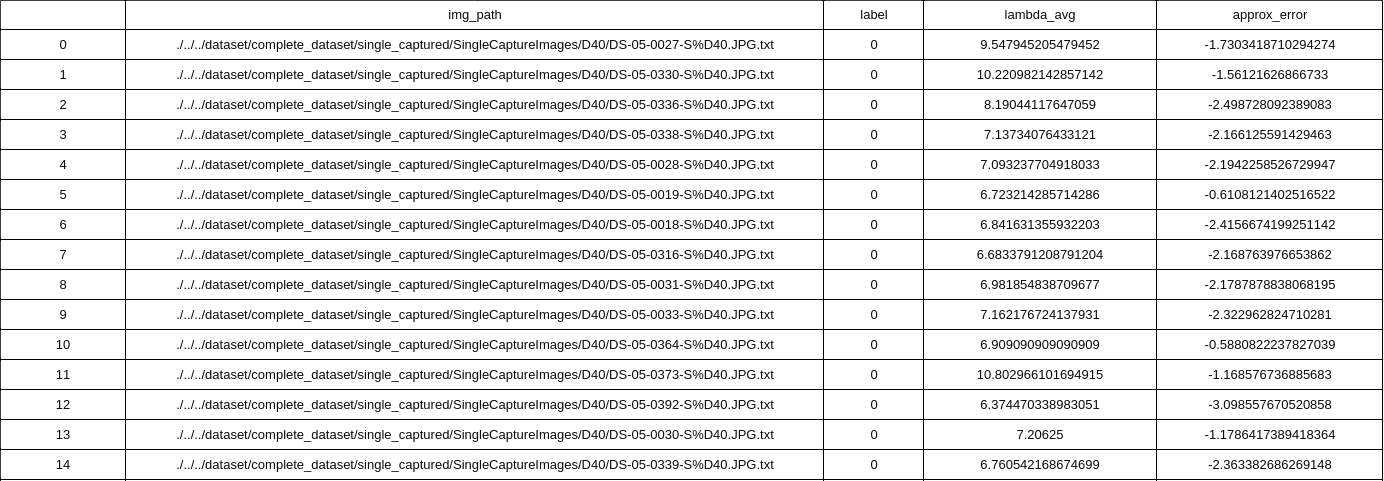
\includegraphics[width=\textwidth]{Images/table.png}
    \caption{Pieces of Panda DataFrame table in .csv file format.}
    \label{fig:table_csv}
\end{figure}

\subsection{Classification}
At this level of implementation, the SVM has already been trained and the model stored.\\
This part of implementation consists of testing the SVM on the test set in order to adress its performances.\\
By analogy with the training phase, this part's explanation is structured in points as well :
\begin{itemize}
    \item the first step consists in extracting the path of all images used for test, both recaptured and single captured, shot by all the cameras;
    \item for each picture, the feature extraction process is performed and the ouput is saved within a .csv file equivalently to the training part;
    \item consequently, a predition is carried out on each image and the results are showed in a table which exhibits: the amount of correctly and erroneously classified rate and the accuracy achieved for each camera model.\\
          Furthermore, the confusion matrix for each camera is video-printed, where :
          \begin{itemize}
              \item the first element represents the True Negatives (images correctly classified as Single Captured);
              \item the first element represents the False Negatives (images wrongly classified as Single Captured);
              \item the first element represents the True Positives (images correctly classified as Recaptured);
              \item the first element represents the False Positives (images wrongly classified as Recaptured);
          \end{itemize}
            It is noteworthy to adress that in order to obtain independent statistics, the classification process is performed separately on each camera model's test set.
\end{itemize}
